\subsection{Interpretador \textit{Tree-Walking}}

Um interpretador é um programa que executa diretamente o código fonte de uma linguagem de programação, linha por linha. No caso deste trabalho, será utilizada a variante \textit{tree-walking}, que simplifica o método de execução do interpretador ao custo de desempenho \cite{craftinginterpreters}. Esta variante se adequa ao objetivo do trabalho, que visa a implementação de um protótipo simples, sem preocupações com desempenho.

A \autoref{fig:mapa_interpretador} ilustra uma montanha fazendo analogia a alguns dos principais caminhos que a implementação de uma linguagem de programação pode seguir. Como será implementado um interpretador \textit{tree-walking} neste trabalho, o caminho pela montanha será o da fase de análise léxica, análise sintática, análise semântica e, por fim, evitando a descida pela montanha, a interpretação direta da representação intermediária gerada pela análise semântica.

\begin{figure}[H]
	\centering
	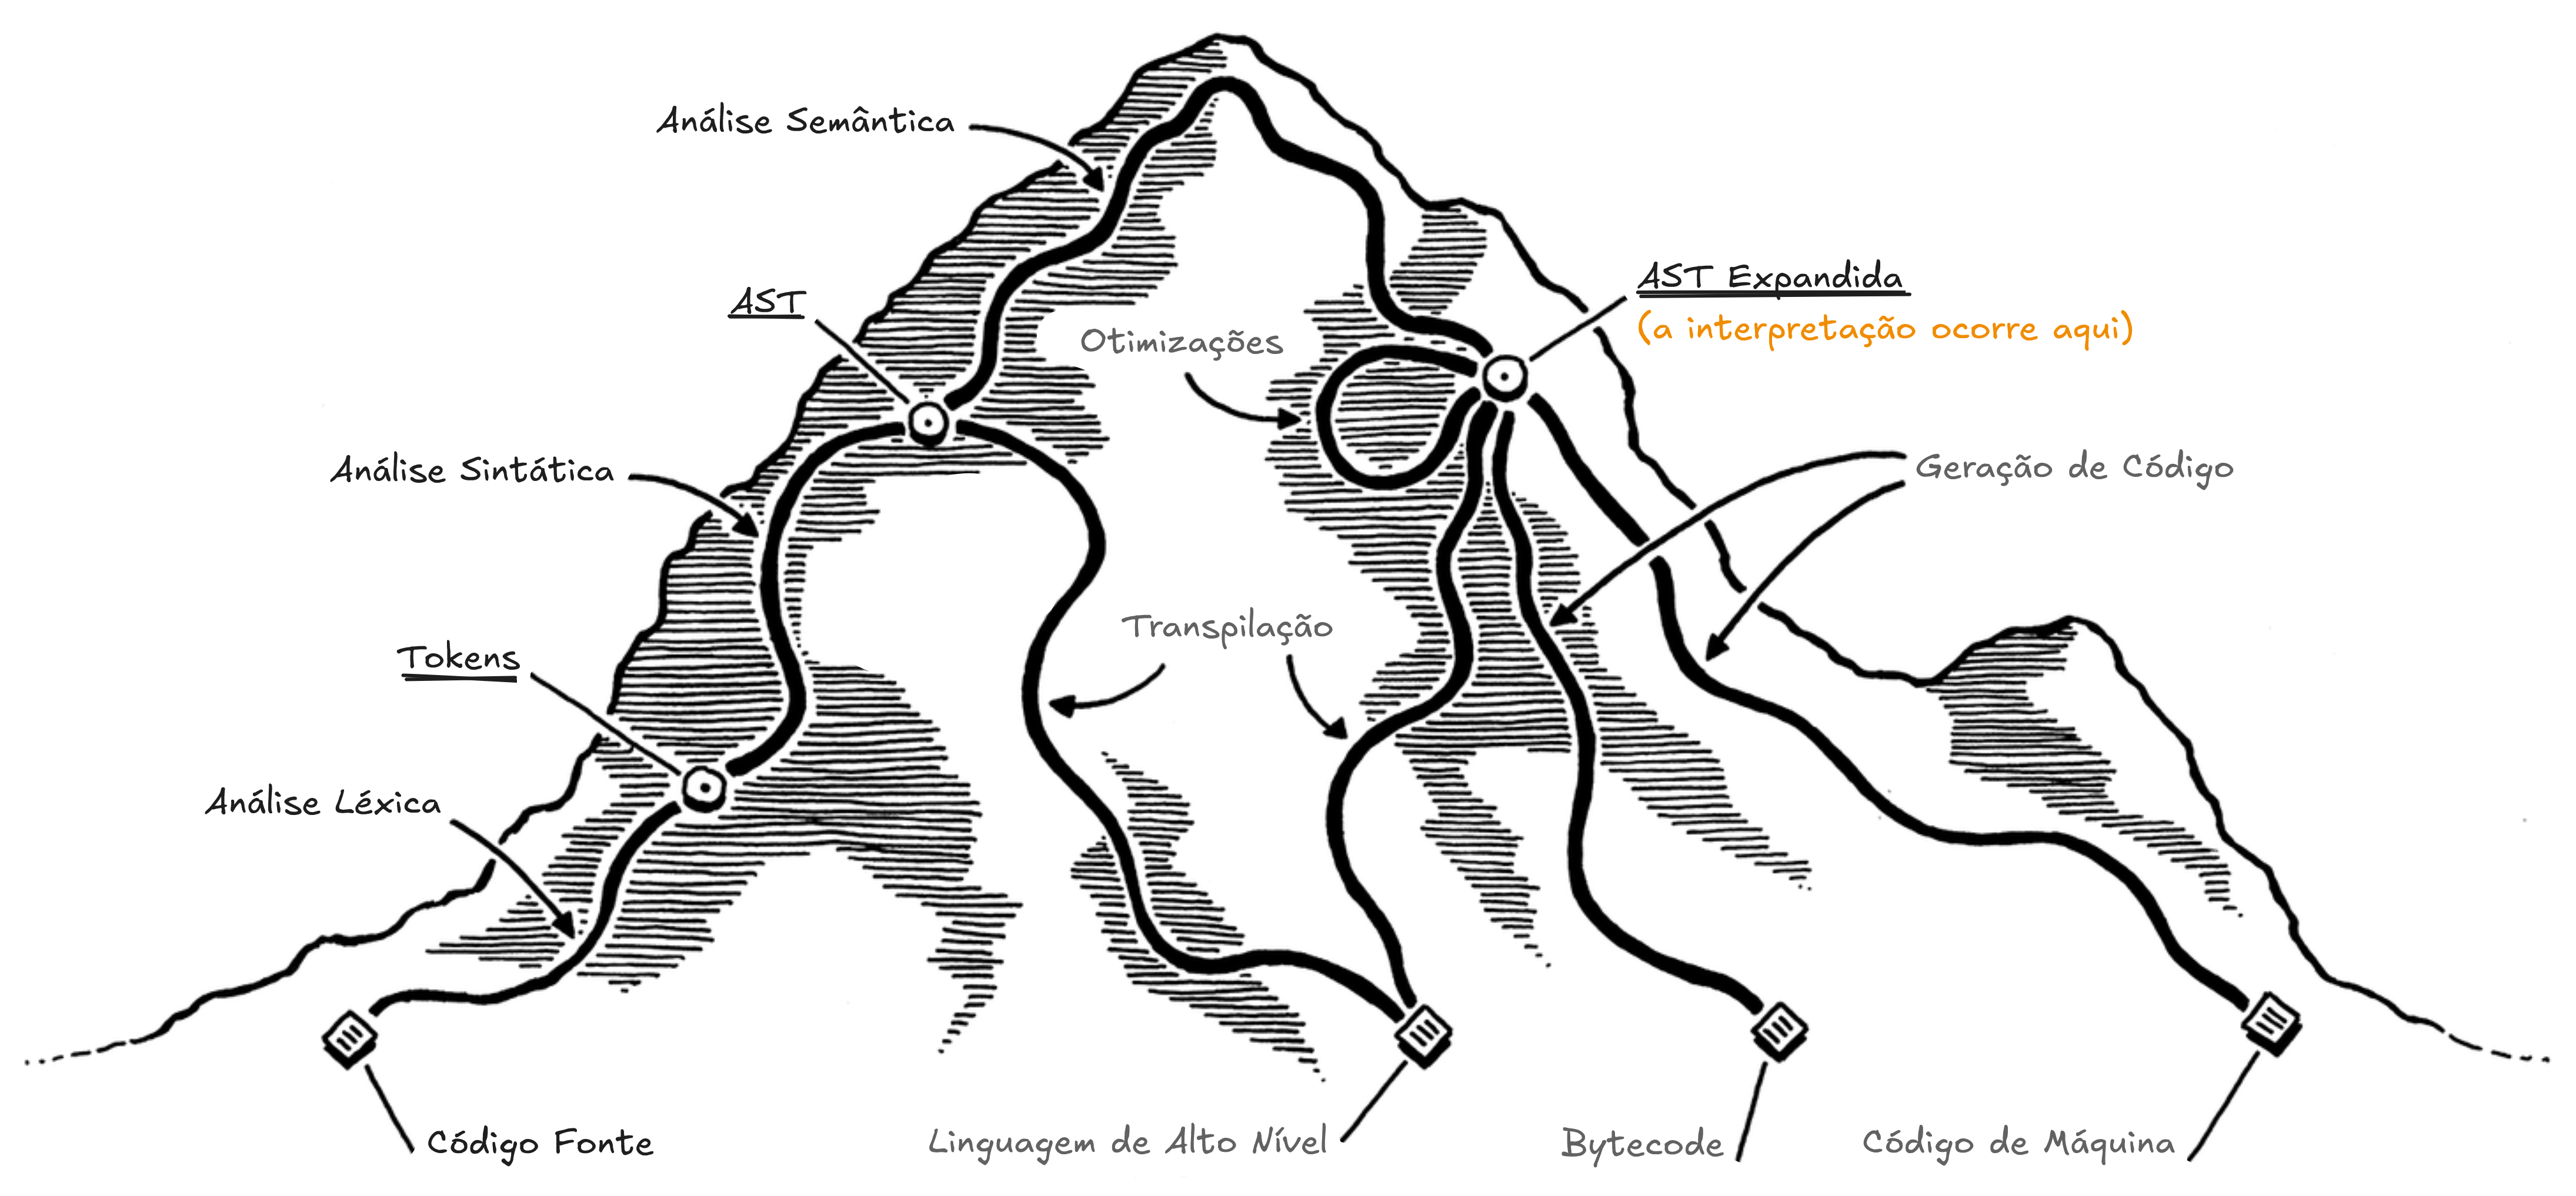
\includegraphics[height=0.3\textheight]{mapa_interpretador}
	\caption{Mapa do território de um interpretador.}
	\fonte{Adaptado de \citeonline{craftinginterpreters}.}
	\label{fig:mapa_interpretador}
\end{figure}

A seguir, serão definidas em detalhe cada uma das quatro principais fases de um interpretador.

\subsubsection{Análise Léxica}

A análise léxica, também conhecida como \textit{lexer}, é a primeira fase do processo de interpretação. Nesta fase, o código fonte é lido e dividido em unidades chamadas \textit{tokens}. Cada \textit{token} representa uma palavra ou símbolo da linguagem de programação, como palavras-chave e operadores. Além disso, cada \textit{token} costuma conter informações adicionais a respeito da palavra, como sua localização ou valor agregado, caso ela possua algum \cite{craftinginterpreters}.

A \autoref{fig:analise_lexica} ilustra o código fonte \texttt{8 + 4 / 2} sendo mapeado para uma lista de \textit{tokens}, onde cada um representa sua determinada palavra do código fonte.

\begin{figure}[H]
	\centering
	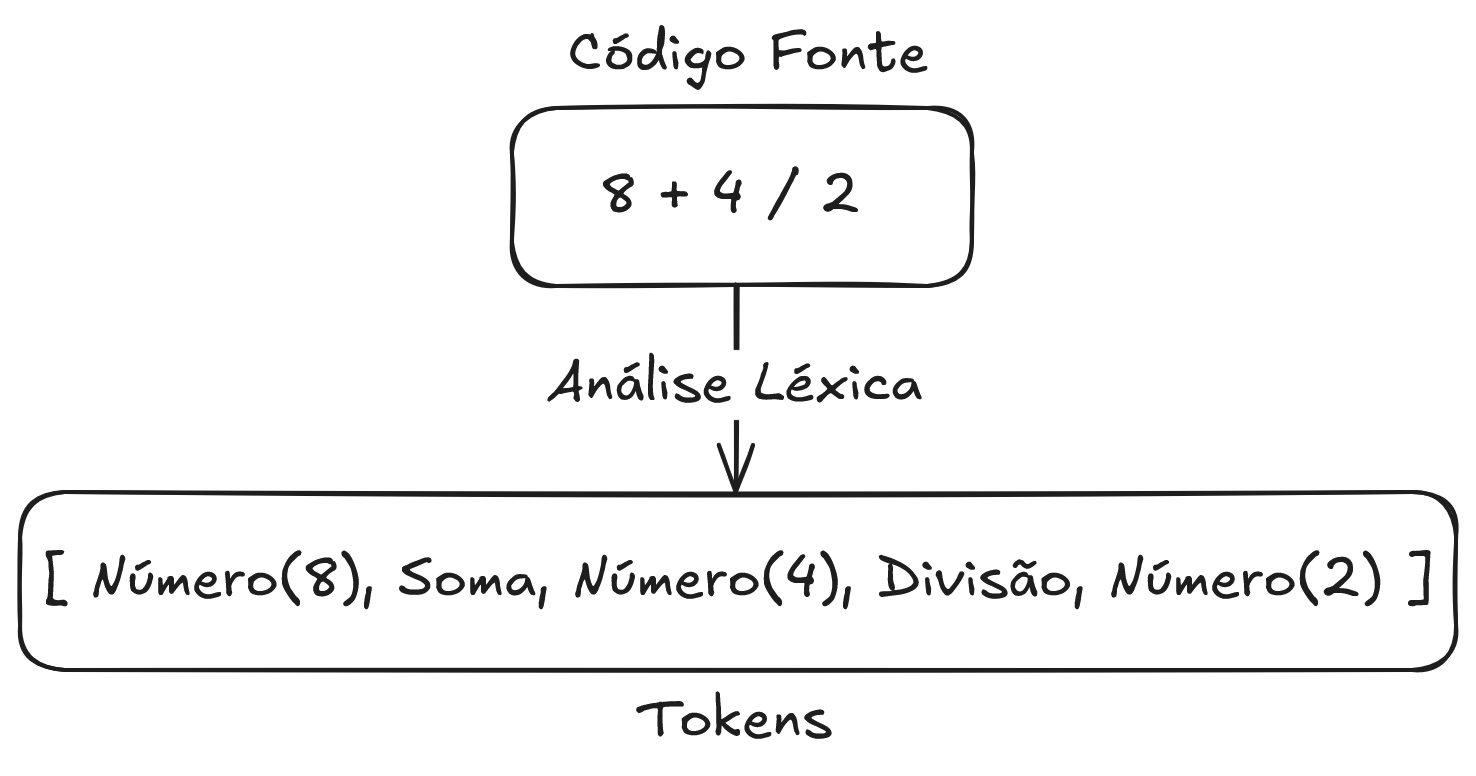
\includegraphics[height=0.2\textheight]{analise_lexica}
	\caption{Código fonte sendo mapeado para uma lista de tokens pela análise léxica.}
	\fonte{Elaboração própria com base em \citeonline{craftinginterpreters}.}
	\label{fig:analise_lexica}
\end{figure}

\subsubsection{Análise Sintática}

A análise sintática, também conhecida como \textit{parser}, é a segunda fase do processo de interpretação. Nesta fase, os \textit{tokens} gerados na fase de análise léxica são organizados em uma estrutura hierárquica chamada árvore sintática abstrata (do inglês, \textit{abstract syntax tree} — AST). A AST representa a estrutura do código fonte de acordo com as regras gramaticais da linguagem de programação \cite{craftinginterpreters}.

A \autoref{fig:analise_sintatica} ilustra a lista de \textit{tokens} sendo mapeada para uma AST, assim gerando a ordem de procedência dos operadores.

\begin{figure}[H]
	\centering
	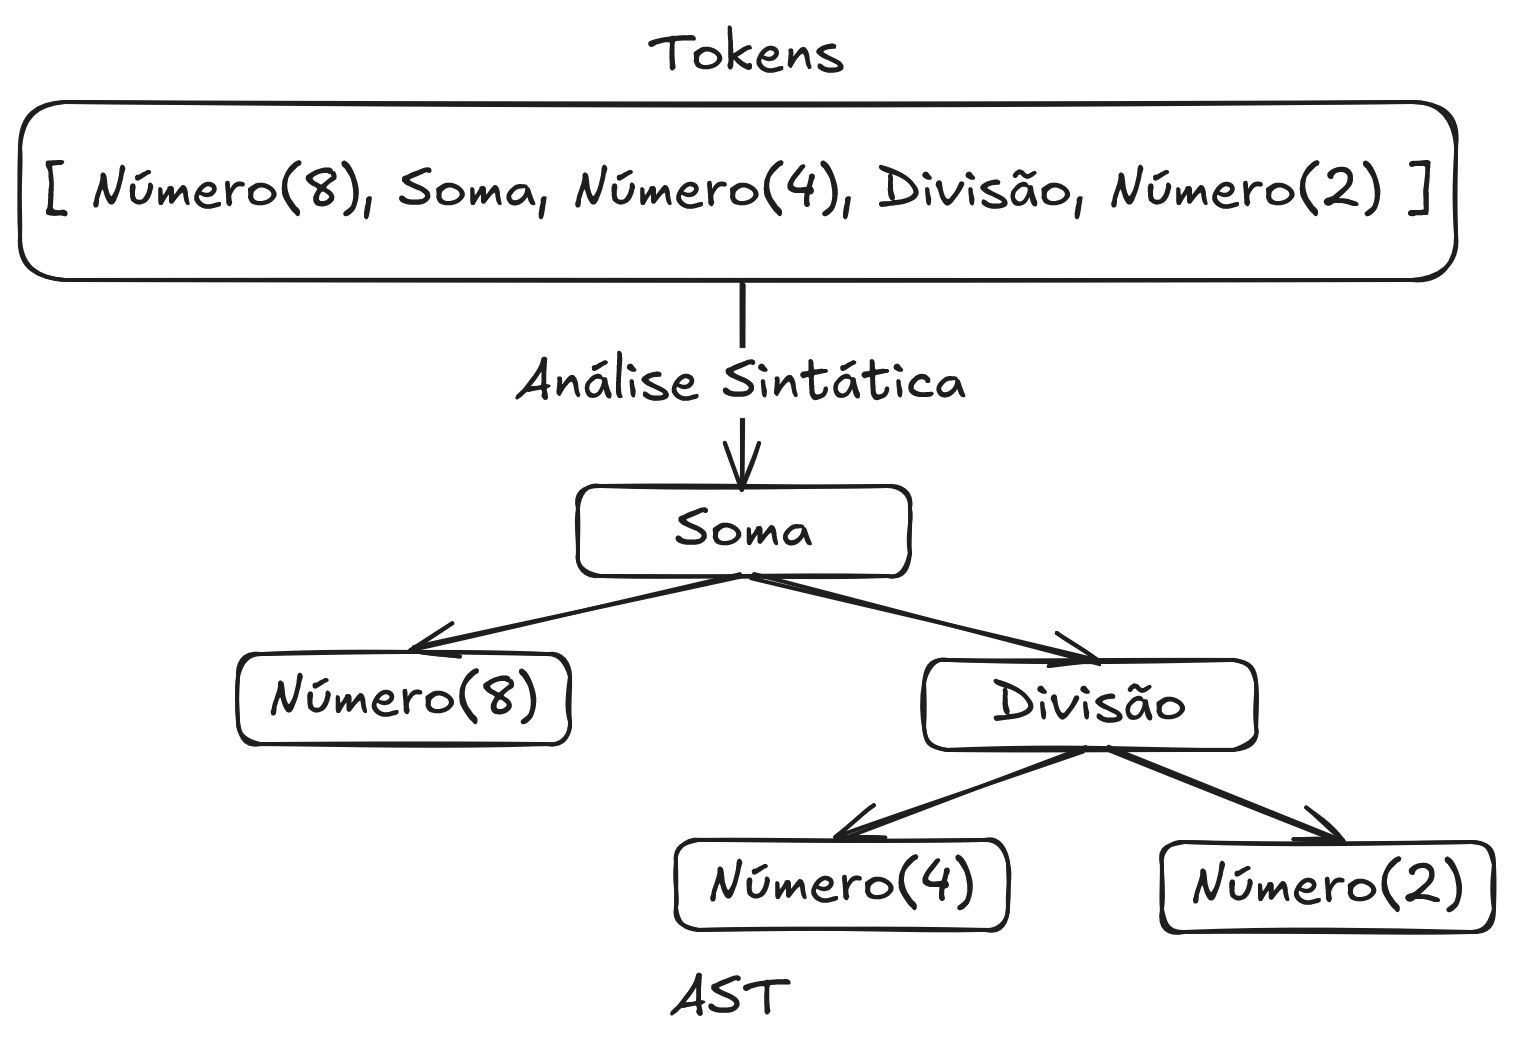
\includegraphics[height=0.27\textheight]{analise_sintatica}
	\caption{Tokens sendo organizados em uma AST pela análise sintática.}
	\fonte{Elaboração própria com base em \citeonline{craftinginterpreters}.}
	\label{fig:analise_sintatica}
\end{figure}

\subsubsection{Análise Semântica}

A análise semântica é uma fase opcional\footnote{Neste trabalho, a análise semântica será implementada.} do processo de interpretação, que visa verificar a consistência e validade do código fonte, além de anotar a AST com informações adicionais, como o tipo de cada expressão \cite{craftinginterpreters}.

Durante esta fase, o interpretador analisa a AST gerada na fase de análise sintática para garantir que as operações e expressões estejam corretas de acordo com as regras da linguagem \cite{craftinginterpreters}. Por exemplo, pode verificar se variáveis foram declaradas antes de serem usadas ou se os tipos de dados são compatíveis.

A \autoref{fig:analise_semantica} ilustra a AST sendo anotada com informações adicionais, como o tipo de cada expressão, resultando em uma AST com mais conhecimento sobre o código fonte.

\begin{figure}[H]
	\centering
	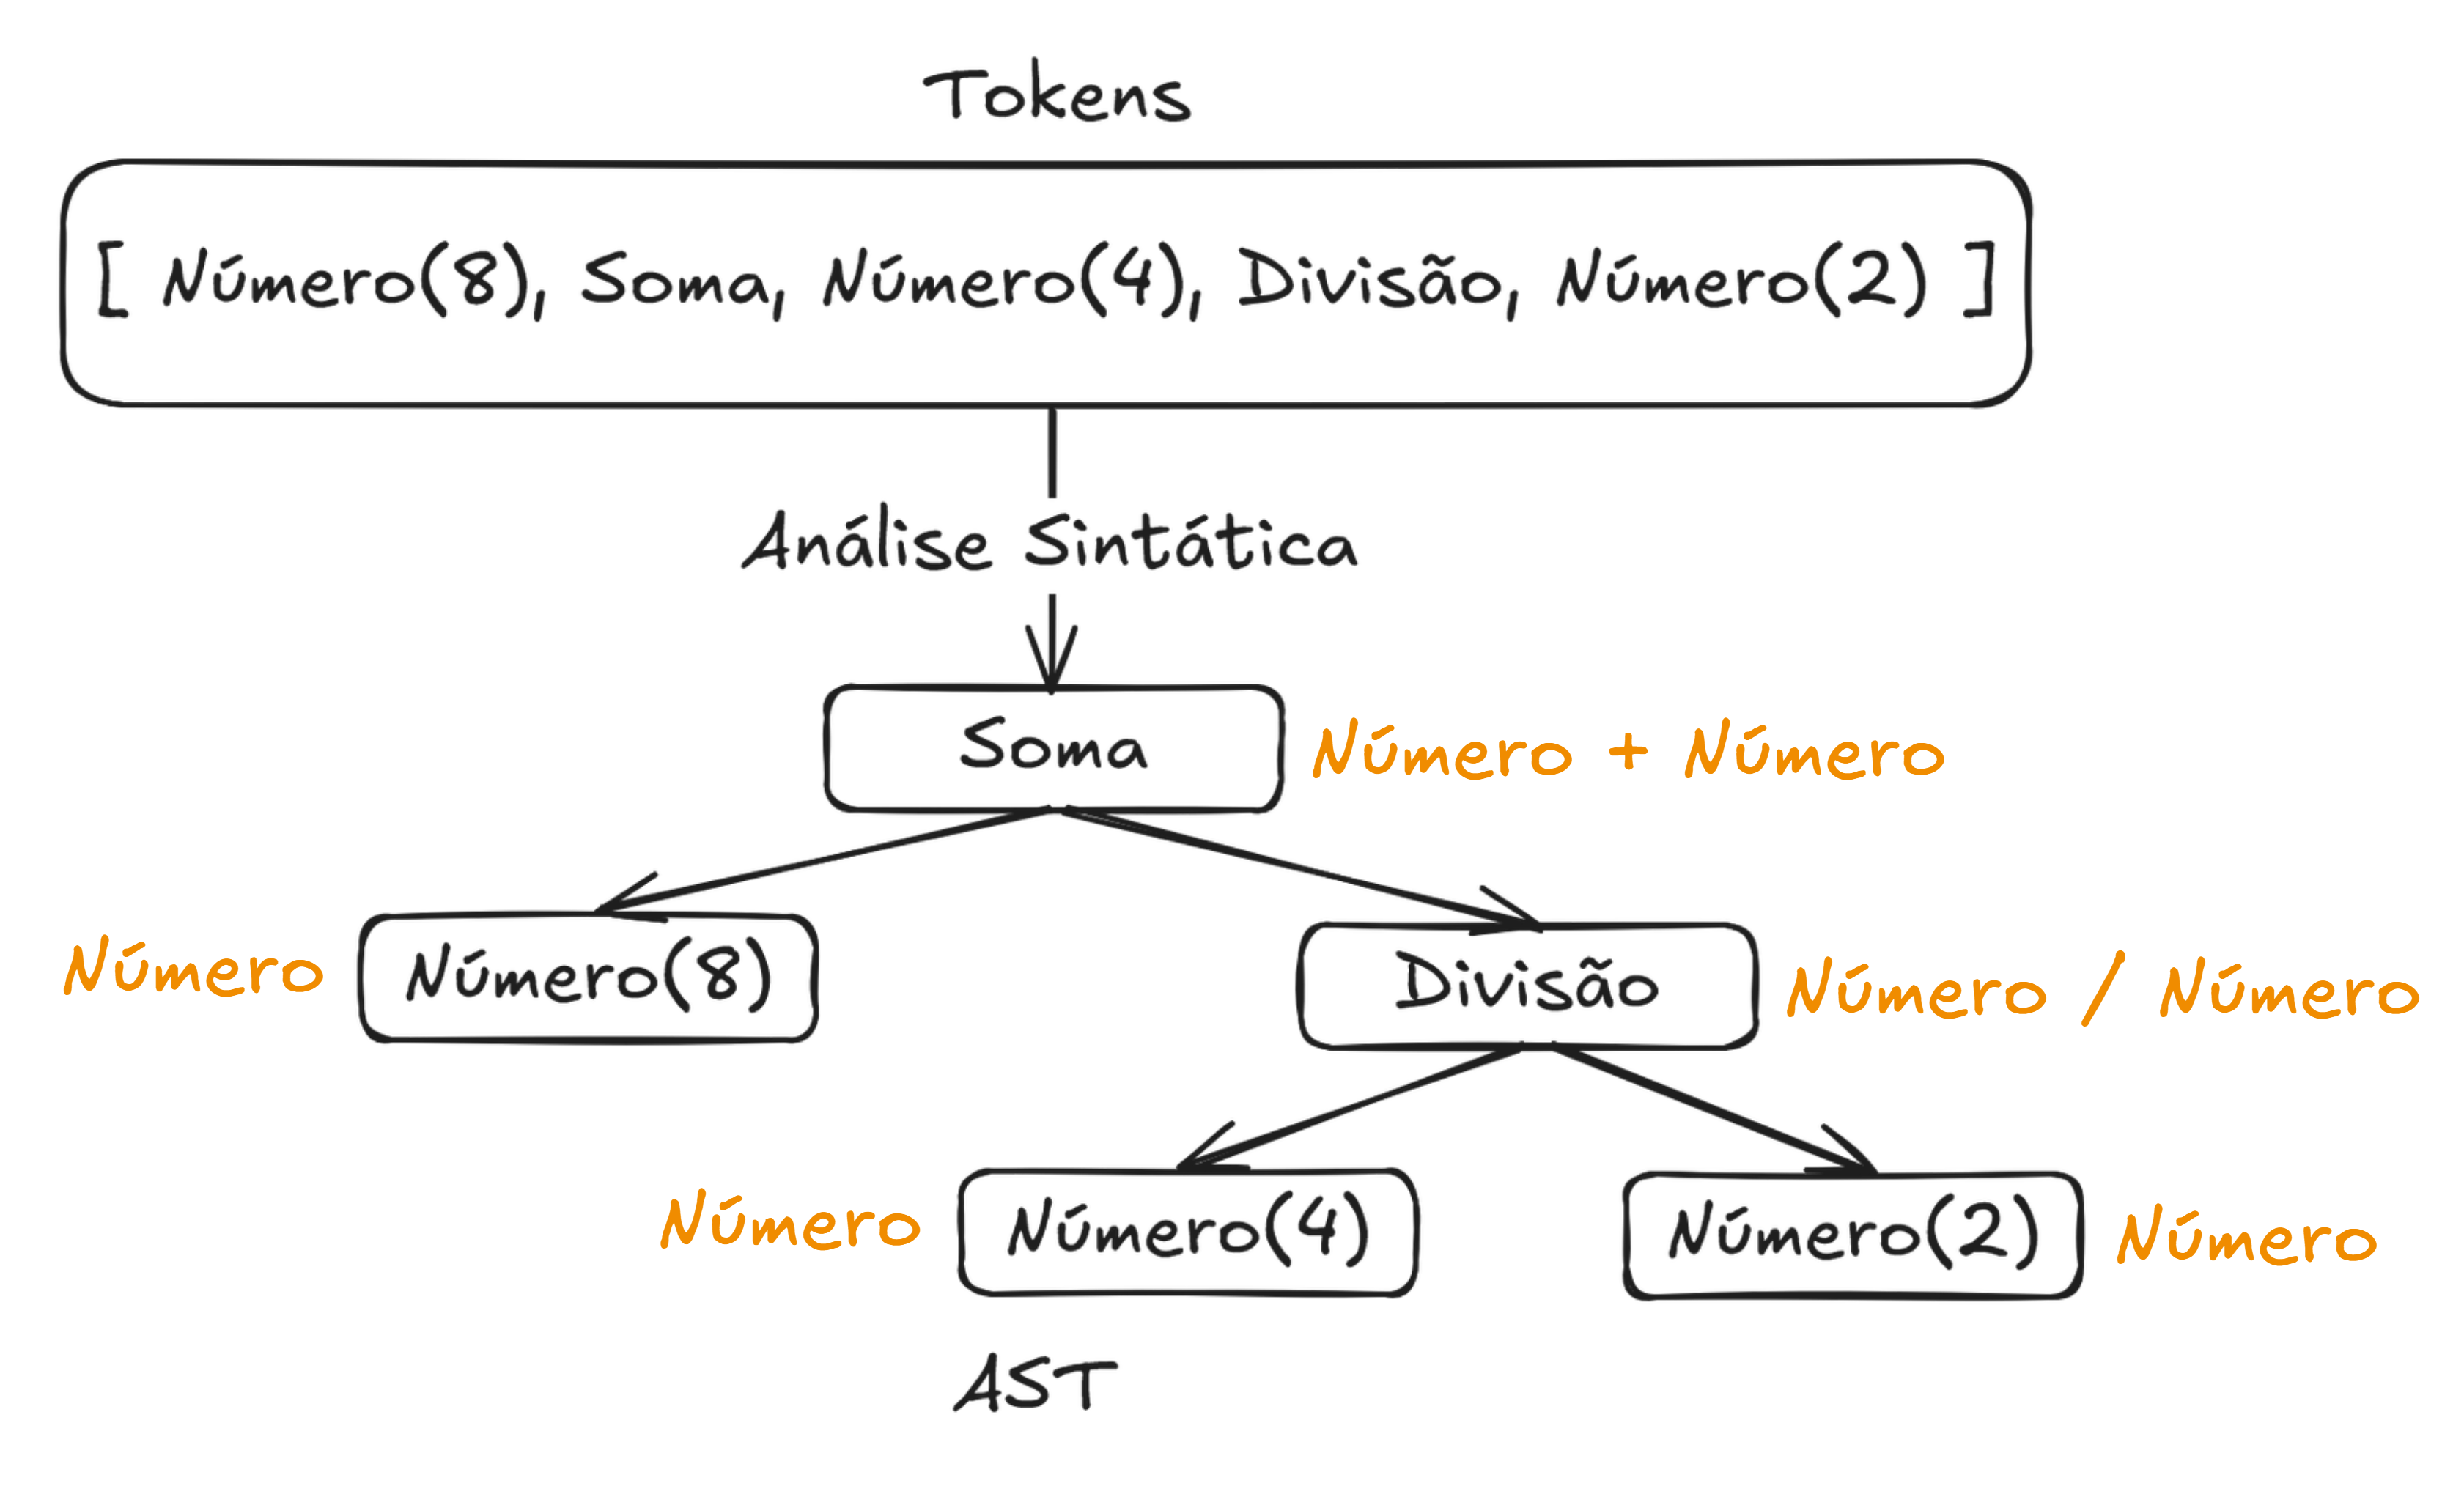
\includegraphics[height=0.27\textheight]{analise_semantica}
	\caption{AST sendo anotada com informações adicionais pela análise semântica.}
	\fonte{Elaboração própria com base em \citeonline{craftinginterpreters}.}
	\label{fig:analise_semantica}
\end{figure}

\subsubsection{Interpretação}

A interpretação é a última fase do processo de interpretação. Nesta fase, a AST gerada na fase de análise sintática e modificada pela análise semântica é percorrida e executada. Durante esta fase, o interpretador avalia expressões, atualiza o estado do programa e executa funções \cite{craftinginterpreters}.

A \autoref{fig:interpretacao} ilustra o processo de interpretação, onde a AST é percorrida e executada pelo interpretador, resultando no número 10.

\begin{figure}[H]
	\centering
	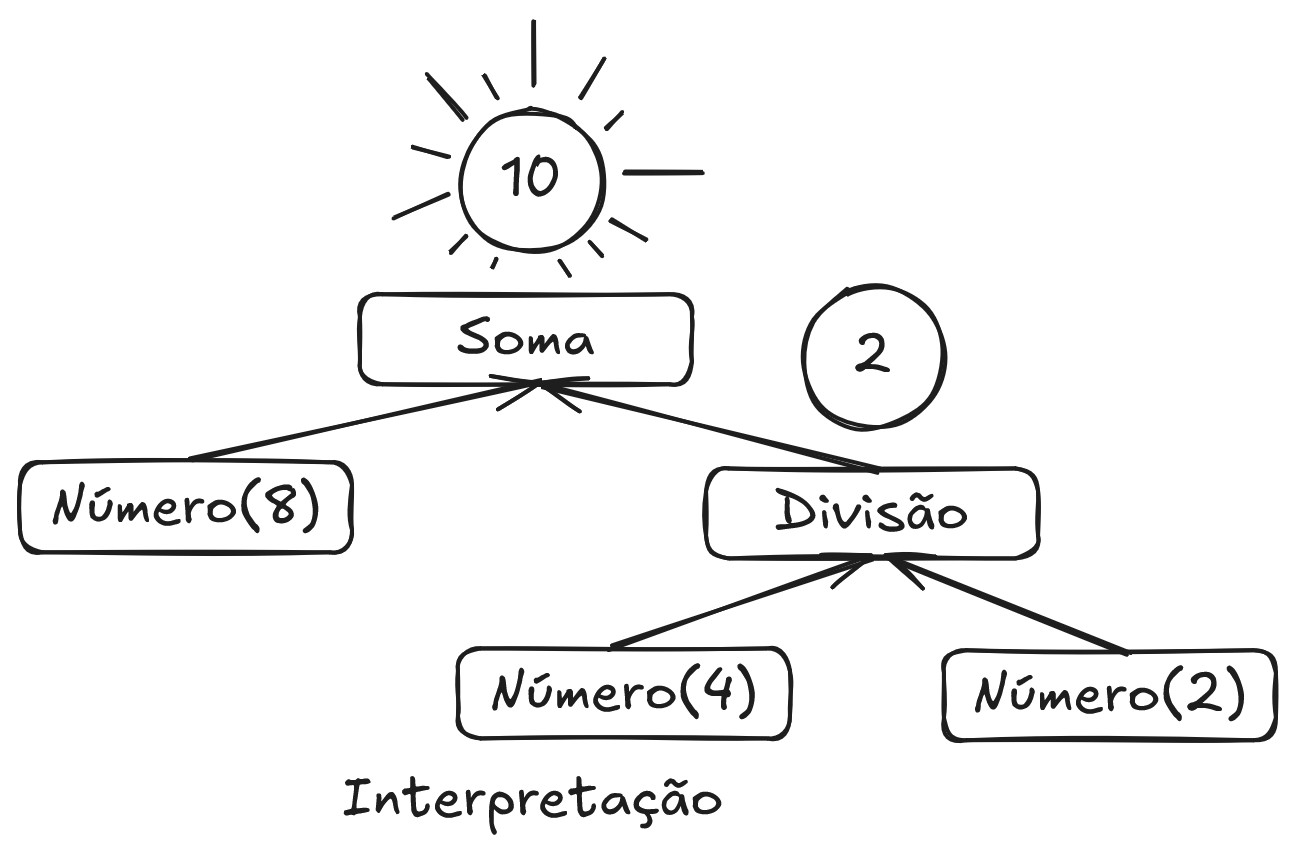
\includegraphics[height=0.25\textheight]{interpretacao}
	\caption{AST sendo percorrida e executada pela fase de interpretação.}
	\fonte{Elaboração própria com base em \citeonline{craftinginterpreters}.}
	\label{fig:interpretacao}
\end{figure}

É importante ressaltar que é na interpretação que o tempo de execução (do inglês, \textit{runtime}) do programa é determinado, pois é quando as expressões são avaliadas e os resultados são produzidos. Em contrapartida, a análise léxica, sintática e semântica são fases de preparação, caracterizando o tempo de compilação (do inglês, \textit{compile time}) do programa.
